%%%%%%%%%%%%%%%%%%%%%%%%%%%%%%%%%%%%%%%%%%%%%%%%%%%%%%%%%%%%%%%
%
% Welcome to Overleaf --- just edit your LaTeX on the left,
% and we'll compile it for you on the right. If you open the
% 'Share' menu, you can invite other users to edit at the same
% time. See www.overleaf.com/learn for more info. Enjoy!
%
%%%%%%%%%%%%%%%%%%%%%%%%%%%%%%%%%%%%%%%%%%%%%%%%%%%%%%%%%%%%%%%

% Inbuilt themes in beamer
\documentclass{beamer}

% Theme choice:
\usetheme{CambridgeUS}
\setbeamertemplate{caption}[numbered]{}

\usepackage{enumitem}
\usepackage{tfrupee}
\usepackage{amsmath}
\usepackage{amssymb}
\usepackage{gensymb}
\usepackage{graphicx}
\usepackage{txfonts}

\def\inputGnumericTable{}

\usepackage[latin1]{inputenc}                                 
\usepackage{color}                                            
\usepackage{array}                                            
\usepackage{longtable}                                        
\usepackage{calc}                                             
\usepackage{multirow}                                         
\usepackage{hhline}                                           
\usepackage{ifthen}
\usepackage{caption} 
\captionsetup[table]{skip=3pt}  
\providecommand{\pr}[1]{\ensuremath{\Pr\left(#1\right)}}
\providecommand{\sbrak}[1]{\ensuremath{{}\left[#1\right]}}
\providecommand{\brak}[1]{\ensuremath{\left(#1\right)}}
\providecommand{\cbrak}[1]{\ensuremath{\left\{#1\right\}}}
\renewcommand{\thetable}{\arabic{table}}
\providecommand{\abs}[1]{\left\vert#1\right\vert}

\let\vec\mathbf


% Title page details: 
\title{AI1110 : Probability and Random Variables}
\subtitle{Assignment 9} 
\author{Mannem Charan(AI21BTECH11019)}
\date{\today}


\begin{document}
% Title page frame
\begin{frame}
    \titlepage 
\end{frame}


% Outline frame
\begin{frame}{Outline}
    \tableofcontents
\end{frame}


% Lists frame
\section{Question}
\begin{frame}{Question}
\textbf{Question Example 8.25:}  In a certain university, $60\%$ of all first-year students are male and $75\%$ of all entering
students graduate. We select at random the records of $299$ males and $101$ females and we find that 168 males and 68 females graduated. Test the hypothesis that the events $B = \cbrak{male}$ and $C = \cbrak{graduate}$ are independent with $\alpha = 0.05$. 


\end{frame}

\section{Solution}
\begin{frame}{Solution}
\textbf{Solution :}
We shall test the hypothesis that two events $B$ and $C$ are independent;\\
             $H_{0}:$
       \begin{align}
           \pr{BC} &= \pr{B}\pr{C} 
       \end{align}
   against, $H_{1}:$
       \begin{align}
          \pr{BC}  \neq \pr{B}\pr{C}
       \end{align}
Given that the probabilities,
        \begin{align}
           \pr{B} &= 0.6\\
           \pr{C} &= 0.75
         \end{align}
\end{frame}

\begin{frame}
Now we will apply chi-square test to the partition consisting of the four events,
             \begin{align}
               A_{1} &= BC\\
              A_{2} &= BC'\\
               A_{3} &= B'C\\
              A_{4} &= B'C'
            \end{align}
     Under the hypothesis $H_{0}$, the components of each of the events $A_{i}$ are independent. Hence,
            \begin{align}
              p_{01} &= \pr{B}\pr{C}\\
                           &= 0.45\\
             p_{02} &= \pr{B}\brak{1-\pr{C}}\\
                          &= 0.15\\
            \end{align}
  \end{frame}

\begin{frame}
             \begin{align}
             p_{03} &= \brak{1-\pr{B}}\pr{C}\\
                          &= 0.3\\
             p_{04} &= \brak{1-\pr{B}}\brak{1-\pr{C}}\\
                          &= 0.1
           \end{align}
where,$p_{0i}$ is probability of event $A_{i}$.\\
  Now according to the chi-square test we will accept $H_{0}$ iff,
           \begin{align}
             \sum_{i=1}^{4}\frac{\brak{k_{i} - np_{0i}}^{2}}{np_{0i}} < \chi_{1-\alpha}^{2}\brak{3}
            \end{align}
The left side of the inequality is known as test statistic$\brak{q}$,
            \begin{align}
               \mathbf{q} &=  \sum_{i=1}^{m}\frac{\brak{\mathbf{k}_{i} - np_{0i}}^{2}}{np_{0i}}
            \end{align}
  where,
        $k_{i}$ is the number of occurences of the event $A_{i}$, $m$ is the no. of classes of the partition and $\chi^{2}\brak{k}$ is chi-square distribution.
\end{frame}

\begin{frame}
In this case,
       \begin{align}
          k_{1} &= 168\\
          k_{2} &= 131\\
          k_{3} &= 68\\
          k_{4} & = 33
       \end{align}
   Now after substituting we will get,
        \begin{align}
           q \approx 4.1
        \end{align}
  And since,
       \begin{align}
           \chi^{2}_{0.95}\brak{3} \approx 7.81 > 4 .1
       \end{align}
  We can accept the independent hypothesis.
\end{frame}

\begin{frame}
        \begin{figure}
           \centering
           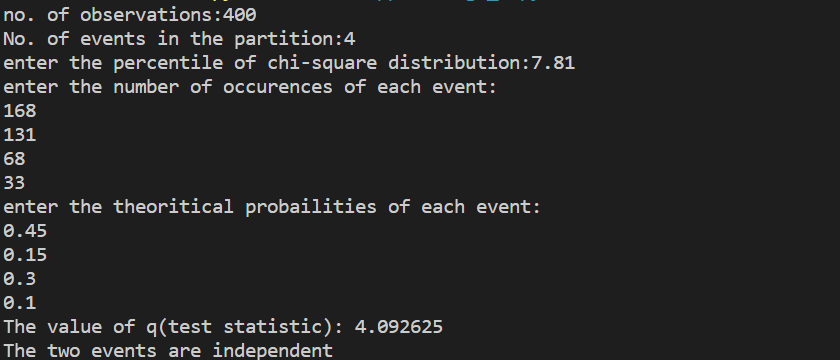
\includegraphics[width = 10cm]{output2.png}
           \caption{Output of python code}
           \label{Figure 1}
         \end{figure}
\end{frame}
 \end{document}         
 